\section{Asynchronous transition systems}
\label{sec:asynchronous-transition-systems}

    Asynchronous transition systems were introduced independently by Bednarczyk \cite{bed88CategoriesAsynchSystems} and Shields \cite{Shields84}. They extend transition systems by including a \emph{binary} independence relation between the occurrence of events. In this model, transitions are events bearing this independence relation. Asynchronous transition systems can be viewed as asynchronous graphs, whose vertices are states and whose edges are transition between states. Transitions take the commutation between events into consideration \cite[Section 3.3]{Fajstrup16DirectedAlgebraicTopologyConcurrency}. If two events commute, then these may be executed at the same time. Meaning that we can consider two transitions of events as a single transition with two events.
    
    \begin{definition}[Asynchronous transition system \cite{winskel95modelsCategory}]\label{def:asynchronous-transition-system}
        An \emph{asynchronous transition system} is a tuple ($\mathcal{S},i,E,\mathcal{I},Tran$) where
        \begin{itemize}
            \item ($\mathcal{S},i,E,Tran$) is a transition system and
            \item $\mathcal{I} \subseteq E \times E$ is an irreflexive symmetric relation, called the independence relation, such that:
            
            \begin{enumerate}
                \item $a \in E \Rightarrow \exists s, s' \in \mathcal{S}, (s,a,s') \in Tran$.
                \item $(s,a,s') \in Tran \wedge (s,a,s'') \in Tran \Rightarrow s' = s''$.
                \item $a\mathcal{I}b \wedge (s_{1},a,s_{2}) \in Tran \wedge (s_{1}, b, s_{3}) \in Tran \Rightarrow \exists u, (s_{2},b,u) \in Tran \wedge (s_{3},a,u) \in Tran$.
                \item $a\mathcal{I}b \wedge (s_{1},a,s_{2}) \in Tran \wedge (s_{2}, b, u) \in Tran \Rightarrow \exists s_{3}, (s_{1},b,s_{3}) \in Tran \wedge (s_{3},a,u) \in Tran$.
            \end{enumerate}
        \end{itemize}
    \end{definition}
    
    Condition (1) says every event should appear as a transition. Condition (2) says that transitions with an event from a state has to be unique, meaning that the transition system should be deterministic. Condition (3) and (4), are pictured respectively in Figure \ref{fig:condition-3-asynchronous-transition-systems} and \ref{fig:condition-4-asynchronous-transition-systems}, exhibiting the transitions of events bearing the independence relation that deals with independent events.
    
    \begin{figure}[ht]
        \centering
        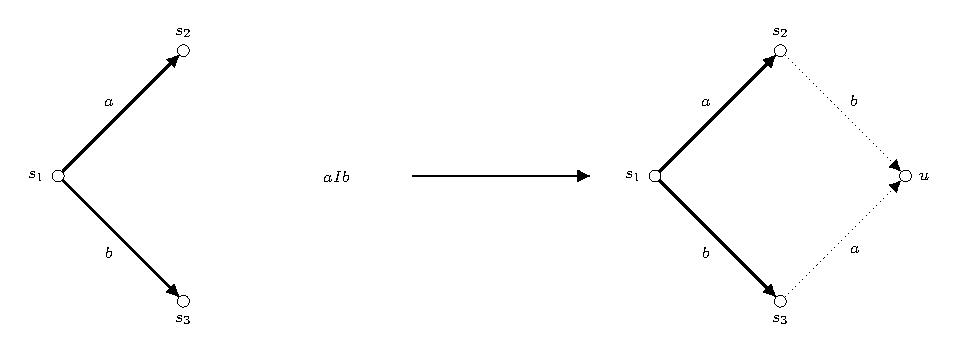
\includegraphics[scale=1]{Figures/2.Models-for-concurrency/Asynchronous-transition-system-condition3.pdf}
         \captionof{figure}[Condition (3) for asynchornous transition systems]{Condition (3) for asynchronous transition systems, where the right-hand side shows how to interpret two independent events coming from a common state. If two events, $a$ and $b$, occur independently from a common state $s$, then they should be able to form the right-hand side.}
        \label{fig:condition-3-asynchronous-transition-systems}
    \end{figure}
    
    \begin{figure}[ht]
        \centering
        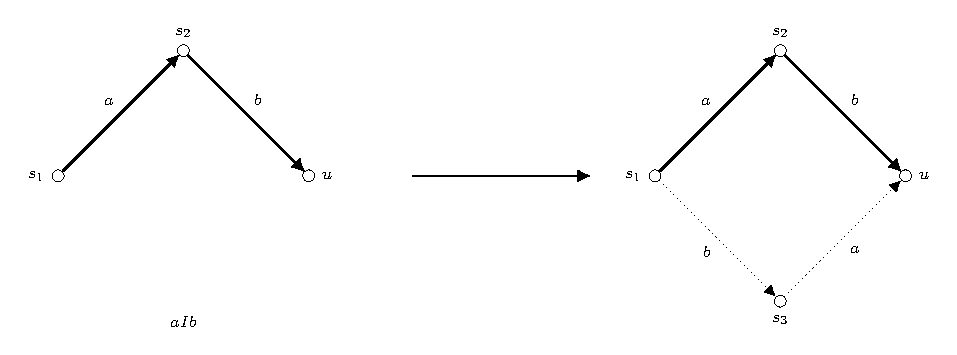
\includegraphics[scale=1]{Figures/2.Models-for-concurrency/Asynchronous-transition-system-condition4.pdf}
        \captionof{figure}[Condition (4) for asynchronous transition systems]{Condition (4) for asynchronous transition systems, where the right-hand side shows how to interpret two independent events occurring immediately after each other. If two events, $a$ and $b$, occur one immediately after the other, then they should be able to occur with their order interchanged.}
        \label{fig:condition-4-asynchronous-transition-systems}
    \end{figure}
    
     Morphisms between asynchronous transition systems are morphisms between their underlying transition systems which preserve the additional relations of independence.
    
    \begin{definition}[Morphisms of asynchronous transition system \cite{winskel95modelsCategory}]\label{def:morphisms-asynchronous-transition-system}
       Let $\mathcal{T} = (\mathcal{S},i,E,\mathcal{I},Tran)$ and $\mathcal{T}^{'} = (\mathcal{S}^{'},i^{'},E^{'},\mathcal{I}^{'},Tran^{'})$ be asynchronous transition systems. A morphism $\mathcal{T} \rightarrow \mathcal{T}^{'}$ is a morphism of transition systems
       
       \begin{center}
            $(\sigma, \lambda) : (\mathcal{S},i,E,Tran) \rightarrow (\mathcal{S}^{'},i^{'},E^{'},Tran^{'})$
       \end{center}
       
       such that
       
       \begin{center}
           $a\mathcal{I}b$ and $\lambda(a), \lambda(b)$ are both defined $\implies$ $\lambda(a)\mathcal{I}\lambda(b)$.
       \end{center}
    \end{definition}
    
    Morphisms of asynchronous transition systems compose as morphisms between their underlying transition systems. We can turn asynchronous transitions systems into a category, written $\allATS$. The category of asynchronous transition systems restricted over the events $E$ is named $\allATS_{E}$.
    
    In interleaving models for concurrency, the number of executions grow exponentially with the size of the program. Every possible execution of a program must be considered, which is not feasible in practice. Non-interleaving models take the commutation of instructions into account, that is, allowing instructions to be executed at the same time. By commuting instructions, it minimizes the number of possible executions of a program by considering certain instructions to be equivalent.
    
    From the independence relation, we can observe that many of the schedules are equivalent in the sense that one can be obtained from the other by permuting independent instructions. Furthermore, such equivalent executions will always lead to the same result. Consequently, if one of those executions can be shown not to lead to an error, neither will any other execution which is equivalent to it.
    
    An independence relation is able to deal directly with concurrency. However, the relation is binary meaning that at most two events can be distinguished. To be able to distinguish an arbitrary number of events, we could extend the independence relation to be an $n$-$ary$ relation. However, this relation should be interpreted as a tractable algebraic theory, which has shown to be challenging.